% !TEX root = main.tex
\documentclass[10pt, twocolumn, a4paper]{article}

% --- Préambule ---
 %!TEX root = main.tex

% --- Encodage et langue ---
\usepackage[utf8]{inputenc}
\usepackage[T1]{fontenc}
\usepackage[french]{babel}

% --- Mise en page ---
\usepackage[margin=2cm]{geometry}
\usepackage{parskip}
\usepackage{booktabs}
\usepackage{multirow}
\usepackage{float}
\usepackage{caption}
\usepackage{setspace}

% --- Graphiques et images ---
\usepackage{graphicx}
\usepackage{wrapfig}
\usepackage{xcolor}
\usepackage[most]{tcolorbox}

% --- Maths ---
\usepackage{amsmath}
\usepackage{amsfonts}

% --- Liens et navigation ---
\usepackage{hyperref}
\hypersetup{
    colorlinks=true,
    linkcolor=black,
    citecolor=blue,
    filecolor=magenta,
    urlcolor=cyan,
    pdftitle={Gesture Recognition Report},
}

\captionsetup{font=small, labelfont=bf, textfont=it}

% --- Couleurs UCLouvain ---
\definecolor{uclgold}{HTML}{C5B36A}
\definecolor{ucllight}{HTML}{E2E86B}

\begin{document}

% --- Page de garde ---
\input{page_de_garde.tex}

\onecolumn
% !TEX root = main.tex
% --- Abstract (single page, single column) ---
\begin{center}
  \begin{minipage}{0.75\textwidth}
    \begin{center}
      \textbf{\large Abstract}
    \end{center}
    \vspace{0.8em}
    \noindent Hand gesture recognition is a central problem in Human--Computer
    Interaction (HCI), where the goal is to classify sequences of three-dimensional
    coordinates $\mathbf{r}(t) = [x(t), y(t), z(t)]^{\top}$ recorded over discrete
    time. This project implements and compares four classifiers on the gesture
    datasets introduced by Huang et al.~\cite{Huang2019}, namely \emph{domain 1}
    (digits 0--9) and \emph{domain 4} (3D figures). Two baseline methods based
    on dynamic programming are first considered: Dynamic Time Warping (DTW)
    and an Edit-distance-based classifier, the latter relying on a preliminary
    vector-quantization step. Two state-of-the-art approaches are then
    investigated: the Three-Cents ($3\mathbb{c}$) recognizer of Caputo et al.~\cite{Caputo2018},
    a rotation-free 3D adaptation of the \$1 recognizer~\cite{Wobbrock2007}, and a Recurrent
    Neural Network (RNN). All methods are evaluated through leave-one-user-out
    (user-independent) and leave-one-gesture-sample-out (user-dependent)
    cross-validation procedures, and compared using hypothesis testing. This
    report details the theoretical framework of each method, the implementation
    strategy, and a rigorous statistical comparison of their accuracies.
  \end{minipage}
\end{center}

\newpage
\twocolumn

\section{Introduction}
\label{sec:introduction}
% !TEX root = main.tex

The development of natural user interfaces has fostered a growing interest in
hand gesture recognition as a means of interaction between humans and machines.
Gestures, being rapidly executed freehand drawings
\cite{Huang2019}, exhibit a strong inherent variability: two instances of the
same gesture produced by the same user may differ in speed, scale, spatial
position, and duration. The sequential nature of the signal and this variability
are the main challenges any recognizer must address.

In this work we consider the problem of classifying three-dimensional gesture
trajectories recorded as a sequence of spatial coordinates. Following the
project guidelines, we assume constant time steps ($t = 1, 2, 3, \dots$) and
ignore the precise sampling instants. Four classifiers are implemented and
compared:
\begin{enumerate}\itemsep 0em
    \item Dynamic Time Warping (DTW) as a first baseline, combined with
    a $k$-nearest-neighbors ($k$-NN) classifier;
    \item Edit-distance on quantized symbolic sequences, as a second
    baseline;
    \item The Three-Cents ($3\mathbb{c}$) recognizer, a 3D extension of the
    \$1 recognizer~\cite{Wobbrock2007};
    \item A Bidirectional Long Short-Term Memory network (BiLSTM) trained end-to-end.
\end{enumerate}

Each method is evaluated on two datasets from~\cite{Huang2019} under both a
\emph{user-independent} and a \emph{user-dependent} cross-validation protocol.
The research questions underlying this project are threefold: (Q1)~\emph{how do
classical template-matching baselines compare with more recent recognizers on
3D mid-air gestures?}; (Q2)~\emph{do user-independent settings systematically
degrade accuracy, as expected?}; and (Q3)~\emph{is one of the investigated
classifiers significantly better than the others in the user-independent
setting?}

The remainder of the report is organized as follows. Section~\ref{sec:data}
describes the datasets. Section~\ref{sec:theory} develops the theoretical
framework of the four methods. Section~\ref{sec:impl} outlines the
implementation and evaluation methodology. Section~\ref{sec:results} presents
and discusses the experimental results, and Section~\ref{sec:conclusion}
concludes.

\section{Data description}
\label{sec:data}
% !TEX root = main.tex

All the data used in this project come from the experiment of
Huang~et~al.~\cite{Huang2019}. The complete dataset comprises four domains of
ten gestures each, each gesture being performed ten times by ten different
subjects, for a total of $10 \times 10 \times 10 = 1000$ samples per domain. In
this work we focus on two of these domains:
\begin{itemize}\itemsep 0em
    \item Domain 1 :  hand-drawn representations of the digits
    $\{0, 1, \dots, 9\}$ in 3D;
    \item Domain 4 : 3D geometric figures.
\end{itemize}

Each gesture is recorded as a finite sequence of 3D position vectors
\begin{equation}
    \mathbf{r}(t) = [x(t), y(t), z(t)]^{\top} \in \mathbb{R}^{3},
    \quad t = 1, 2, \dots, T_i ,
\end{equation}
where $T_i$ is the length of the $i$-th sample and may vary across recordings.
As stated in the project guidelines, the discrete time index is treated as
uniform, even though this assumption is not strictly satisfied in practice.


% ================================================================
\section{Theoretical framework}
\label{sec:theory}
% !TEX root = main.tex
% ================================================================

This section introduces the four methods used in our comparative study. We
first describe the two dynamic-programming baselines (DTW and Edit-distance),
then the Three-Cents recognizer, and finally the BiLSTM.
Throughout, we denote the test sequence by
$\mathcal{X} = (\mathbf{x}_1, \dots, \mathbf{x}_N)$ and a reference (template)
sequence by $\mathcal{Y} = (\mathbf{y}_1, \dots, \mathbf{y}_M)$, with
$\mathbf{x}_i, \mathbf{y}_j \in \mathbb{R}^{3}$.

% ----------------------------------------------------------------
\subsection{Dynamic Time Warping (DTW)}
% ----------------------------------------------------------------

Dynamic Time Warping is a classical technique for comparing two time-dependent
sequences that may differ in speed or duration
\cite{MyersRabiner1981}. The key idea is to find a non-linear
alignment between the two sequences that minimizes a cumulative distance,
thereby absorbing local temporal distortions.

We first define the local cost between two points $\mathbf{x}_i$ and
$\mathbf{y}_j$ via the Euclidean ($L_2$) distance:
\begin{equation}
    d(i, j) = \lVert \mathbf{x}_i - \mathbf{y}_j \rVert_2 .
\end{equation}

The accumulated distance $D(i, j)$ is then computed recursively using dynamic
programming~\cite{Rabiner1993}:
\begin{equation}
\label{eq:dtw-recurrence}
    D(i, j) = d(i, j) + \min
    \begin{cases}
        D(i-1, j-1) \\[2pt]
        D(i-1, j)   \\[2pt]
        D(i, j-1)
    \end{cases}
\end{equation}
with boundary condition $D(1, 1) = d(1, 1)$. The three candidate predecessors
correspond respectively to a diagonal step (temporal alignment), a vertical
step (the test sequence is progressing while the reference is stalling), and a
horizontal step (the reference is progressing while the test is stalling).

A warping path $W = (w_1, \dots, w_L)$, with $w_k = (i_k, j_k)$, is a sequence
of grid cells traversed from $(1,1)$ to $(N, M)$. To be physically meaningful,
$W$ must satisfy three standard constraints~\cite{Rabiner1993}:
\begin{itemize}\itemsep 0em
    \item Boundary: $w_1 = (1, 1)$ and $w_L = (N, M)$;
    \item Monotonicity: both index sequences $(i_k)$ and $(j_k)$ are
    non-decreasing (temporal order is preserved);
    \item Continuity: transitions occur only between adjacent cells, so
    that no observation is skipped.
\end{itemize}

The final similarity score $D(N, M)$ is then plugged into a $k$-nearest-neighbors classifier: the
test gesture is assigned the majority label among its $k$ closest templates.

% ----------------------------------------------------------------
\subsection{Edit-distance on quantized sequences}
% ----------------------------------------------------------------
The second baseline treats gestures as strings of discrete symbols and
classifies them using an edit-distance. The approach proceeds in two steps.
 
\paragraph{Vector quantization.} Each 3D point $\mathbf{r}(t)$ is first assigned
to one of $K$ codewords obtained by clustering the pooled training points
(via $k$-means). A gesture is thereby mapped onto a sequence of discrete
symbols $s(t) \in \{1, \dots, K\}$, turning the continuous trajectory problem
into a string-matching problem. This discretization step is necessary because
edit-distance is fundamentally a string-based metric, designed to compare
sequences of discrete elements rather than continuous coordinates.
 
\paragraph{Edit distance.} The dissimilarity between two such symbolic sequences
is measured by the Levenshtein edit distance~\cite{Levenshtein1966}, defined as
the minimum number of elementary edit operations (insertion, deletion,
substitution) required to transform one sequence into the other:
\begin{equation}
    d_{\text{ED}}(S_1, S_2) = \min \left\{ \text{cost of operations to transform } S_1 \to S_2 \right\} .
\end{equation}
 
The distance is computed using a standard dynamic-programming recursion. Let
$D(i, j)$ denote the edit distance between the first $i$ symbols of $S_1$ and
the first $j$ symbols of $S_2$. Then:
\begin{equation}
    D(i, j) = \min
    \begin{cases}
        D(i-1, j) + 1 & \text{(deletion)} \\[2pt]
        D(i, j-1) + 1 & \text{(insertion)} \\[2pt]
        D(i-1, j-1) + c(i, j) & \text{(substitution)}
    \end{cases}
\end{equation}
where $c(i, j) = 0$ if $S_1[i] = S_2[j]$, and $c(i, j) = 1$ otherwise. The
final value $D(|S_1|, |S_2|)$ gives the edit distance between the two complete
sequences. Classification is performed with a $k$-nearest-neighbors rule,
assigning each test gesture the label of its $k$ nearest templates in the
edit-distance metric.


% ----------------------------------------------------------------
\subsection{The Three-Cents recognizer}
% ----------------------------------------------------------------

The Three-Cents recognizer is a 3D specialization of the \$1 recognizer of
Wobbrock, Wilson and Li~\cite{Wobbrock2007}. The original \$1 algorithm is a
widely used gold standard for 2D gesture prototyping, relying on four steps:
\emph{resample}, \emph{rotate to a reference angle}, \emph{scale}, and
\emph{translate to the origin}, followed by template matching. While effective,
its iterative rotation search (Golden-Section Search) becomes computationally
expensive and geometrically ambiguous in 3D, where no single reference angle
exists.

Caputo et al.~\cite{Caputo2018} propose to forgo the rotation step altogether,
yielding a lightweight three-step normalization pipeline
(\emph{resample--scale--translate}) that remains robust for short mid-air
trajectories.

\subsubsection*{Three-step normalization pipeline}
 
\begin{enumerate}\itemsep 0em
    \item \textbf{Resampling.} The raw trajectory is resampled into $n$
    equidistant points along its arc length (typically $n = 64$, as in the
    original \$1 paper). This makes the representation invariant to the
    execution speed.
 
    \item \textbf{Scaling.} The resampled gesture is rescaled using a
    uniform scaling by total arc length. Let $L$ denote the total
    arc-length of the resampled trajectory:
    \begin{equation}
        L = \sum_{i=1}^{n-1} \lVert \mathbf{r}'_{i+1} - \mathbf{r}'_{i} \rVert_2 .
    \end{equation}
    Following~\cite{Caputo2018}, each point is then divided by $L$:
    \begin{equation}
        \mathbf{r}''_i = \frac{\mathbf{r}'_i}{L} .
    \end{equation}
    This choice differs from the bounding-box scaling used in the original
    \$1 algorithm, which stretches each axis independently and can distort
    the gesture shape. Uniform length-based scaling preserves the
    proportions of the trajectory, making two gestures of the same shape but
    different sizes comparable while preserving directional information
    (crucial for 3D mid-air gestures where orientation is
    discriminative)~\cite{Caputo2018}.
 
    \item \textbf{Translation.} Finally, the gesture is translated so that its
    centroid lies at the origin (0, 0, 0),
    \begin{equation}
        \mathbf{r}_{c} = \tfrac{1}{n} \sum_{i=1}^{n} \mathbf{r}'_i ,
        \qquad
        \mathbf{r}^{\text{final}}_{i} = \mathbf{r}'_i - \mathbf{r}_{c} ,
    \end{equation}
    ensuring position invariance.
\end{enumerate}

\subsubsection*{Classification}

After normalization, the candidate gesture $C = (\mathbf{c}_1, \dots,
\mathbf{c}_n)$ is compared to each template $T = (\mathbf{t}_1, \dots,
\mathbf{t}_n)$ by the average Euclidean point-to-point distance:
\begin{equation}
    D(C, T) = \frac{1}{n} \sum_{i=1}^{n}
    \lVert \mathbf{c}_i - \mathbf{t}_i \rVert_2 .
\end{equation}
A 1-Nearest-Neighbor rule is then applied: the candidate is assigned the label
of the template achieving the minimum distance. By omitting the rotation step
and relying on a fixed point-to-point correspondence, the Three-Cents
recognizer provides a ``cheap'' alternative to alignment-based methods such as
DTW, at the cost of sensitivity to global rotations.

% ----------------------------------------------------------------
\subsection{Bidirectional LSTM}
\label{sec:bilstm}
% ----------------------------------------------------------------

Unlike the previous methods, which are distance-based, the last approach
relies on a recurrent neural network that learns its representation directly
from the data. Recurrent Neural Networks (RNNs) process a sequence
$\mathcal{X} = (\mathbf{x}_1, \dots, \mathbf{x}_T)$ by maintaining a hidden
state that propagates information forward in time. Standard RNNs trained by
back-propagation through time suffer however from the
\emph{vanishing/exploding gradient problem}: the influence of an early time
step on the loss decays (or blows up) exponentially with the temporal
distance, making it practically impossible to learn long-range dependencies
\cite{Hochreiter1997, Goodfellow2016}. Since a gesture trajectory typically
spans several dozens of frames whose global shape is the primary
discriminating cue, this is a critical limitation.

\subsubsection*{LSTM cell}

The Long Short-Term Memory (LSTM) cell of Hochreiter and
Schmidhuber~\cite{Hochreiter1997} addresses this issue through an internal
\emph{cell state} $\mathbf{c}_t$, regulated by three multiplicative gates.
At each time step $t$, given the input $\mathbf{x}_t$ and the previous
hidden state $\mathbf{h}_{t-1}$:
\begin{align}
    \mathbf{f}_t &= \sigma(\mathbf{W}_f \mathbf{x}_t + \mathbf{U}_f \mathbf{h}_{t-1} + \mathbf{b}_f), \\
    \mathbf{i}_t &= \sigma(\mathbf{W}_i \mathbf{x}_t + \mathbf{U}_i \mathbf{h}_{t-1} + \mathbf{b}_i), \\
    \mathbf{o}_t &= \sigma(\mathbf{W}_o \mathbf{x}_t + \mathbf{U}_o \mathbf{h}_{t-1} + \mathbf{b}_o), \\
    \tilde{\mathbf{c}}_t &= \tanh(\mathbf{W}_c \mathbf{x}_t + \mathbf{U}_c \mathbf{h}_{t-1} + \mathbf{b}_c), \\
    \mathbf{c}_t &= \mathbf{f}_t \odot \mathbf{c}_{t-1} + \mathbf{i}_t \odot \tilde{\mathbf{c}}_t, \\
    \mathbf{h}_t &= \mathbf{o}_t \odot \tanh(\mathbf{c}_t),
\end{align}
where $\sigma$ is the logistic sigmoid, $\odot$ the element-wise product,
and $\{\mathbf{W}_\bullet, \mathbf{U}_\bullet, \mathbf{b}_\bullet\}$ are the
learned parameters. The \emph{forget gate} $\mathbf{f}_t$ controls how
much of the previous cell state is preserved, the \emph{input gate}
$\mathbf{i}_t$ how much of the candidate $\tilde{\mathbf{c}}_t$ is written
to the new state, and the \emph{output gate} $\mathbf{o}_t$ how much of the
cell state is exposed as output. The additive update of $\mathbf{c}_t$
creates a \emph{constant error carrousel} through which gradients can flow
unattenuated across many time steps, which is the key mechanism that
overcomes the vanishing gradient problem~\cite{Hochreiter1997}.
Figure~\ref{fig:lstm-cell} summarizes the cell's internal data flow.

\begin{figure}[t]
    \centering
    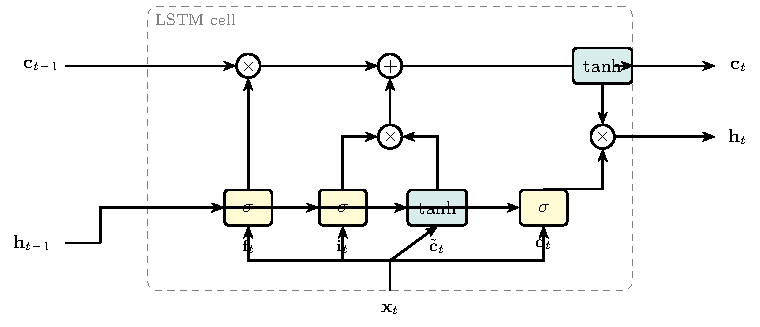
\includegraphics[width=\columnwidth]{figures/lstm_cell.pdf}
    \caption{Internal data flow of an LSTM cell. Three sigmoid gates
    ($f_t, i_t, o_t$) and one $\tanh$ candidate ($\tilde{c}_t$) jointly
    update the cell state $\mathbf{c}_t$ and produce the hidden state
    $\mathbf{h}_t$. The horizontal line carrying $\mathbf{c}_t$ acts as a
    gradient highway, enabling learning over long sequences.}
    \label{fig:lstm-cell}
\end{figure}

\subsubsection*{Bidirectional extension}

A unidirectional LSTM reads the sequence from left to right and classifies
the gesture using only the causal context up to the current frame. Since
gesture recognition is an offline task, the full trajectory is available
before any decision is made, this is unnecessarily restrictive. The
Bidirectional RNN of Schuster and Paliwal~\cite{Schuster1997} runs two
independent recurrent layers in opposite directions and concatenates their
hidden states:
\begin{equation}
    \overrightarrow{\mathbf{h}}_t = \mathrm{LSTM}_{\!\rightarrow}(\mathbf{x}_1, \dots, \mathbf{x}_t),
    \;\;
    \overleftarrow{\mathbf{h}}_t = \mathrm{LSTM}_{\!\leftarrow}(\mathbf{x}_T, \dots, \mathbf{x}_t),
\end{equation}
\begin{equation}
    \mathbf{H}_t = \left[\, \overrightarrow{\mathbf{h}}_t \,;\, \overleftarrow{\mathbf{h}}_t \,\right] \in \mathbb{R}^{2h}.
\end{equation}
Each frame is thus encoded with access to the \emph{entire} temporal
context. This is particularly useful when the beginning of a digit is
ambiguous before its closing stroke is observed (e.g., a 0 versus a 6, or
a 3 versus an 8). In our implementation each direction has $h$ hidden units
(hyperparameter \texttt{n\_units}), and only the final concatenated state
$\mathbf{H}_T$ is forwarded to the classifier head (\texttt{return\_sequences=False}).

\subsubsection*{Classifier head}

The state $\mathbf{H}_T$ is passed through a small feed-forward classifier
illustrated in Figure~\ref{fig:bilstm-arch}. Two regularization mechanisms
are applied first. \emph{Batch normalization}~\cite{Ioffe2015} rescales
each feature of $\mathbf{H}_T$ to zero mean and unit variance over the
mini-batch $\mathcal{B}$, before applying a learned affine transformation:
\begin{equation}
    \hat{y}_k = \gamma_k \,\frac{y_k - \mu_{\mathcal{B},k}}{\sqrt{\sigma^2_{\mathcal{B},k} + \varepsilon}} + \beta_k.
\end{equation}
This reduces the \emph{internal covariate shift} caused by changing
upstream weights during training, stabilizes optimization, and allows
slightly higher learning rates. \emph{Dropout}~\cite{Srivastava2014} is
then applied with rate $p = 0.30$: during training only, each activation
is independently set to zero with probability $p$, forcing the network to
learn redundant representations and acting as an implicit ensemble of
thinned sub-networks. The resulting vector is mapped through a dense layer
of $32$ ReLU units, then to a softmax over the $K = 10$ classes producing
a valid probability distribution
$p_k = e^{z_k} / \sum_{j} e^{z_j}$.

\begin{figure}[t]
    \centering
    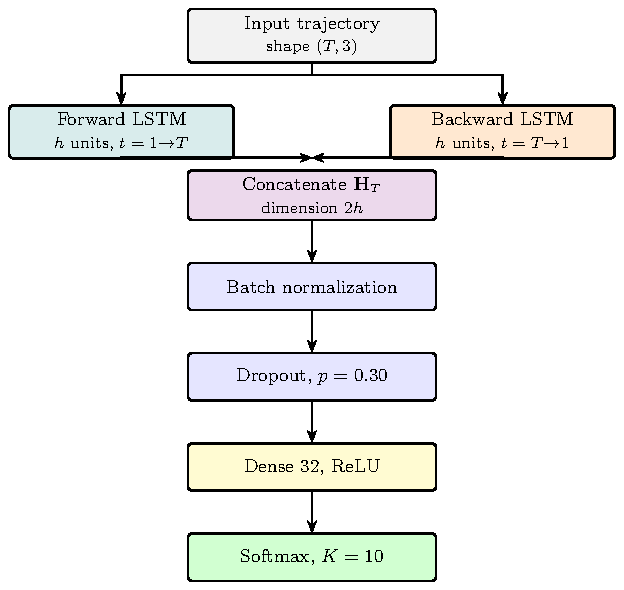
\includegraphics[width=\columnwidth]{figures/bilstm_architecture.pdf}
    \caption{Architecture of the BiLSTM classifier. The trajectory
    (resampled to $T$ points) is processed by two LSTM layers reading in
    opposite directions; their final hidden states are concatenated into
    $\mathbf{H}_T \in \mathbb{R}^{2h}$ and passed through a regularized
    classifier head producing a softmax over the $K = 10$ gesture classes.}
    \label{fig:bilstm-arch}
\end{figure}

\subsubsection*{Training}

The network is trained by minimizing the categorical cross-entropy
\begin{equation}
    \mathcal{L} = -\sum_{k=1}^{K} y_k \log p_k ,
\end{equation}
where $\mathbf{y}$ is the one-hot encoded label. Optimization uses
Adam~\cite{Kingma2015}, an adaptive first-order method that maintains
exponentially decaying estimates of the first ($\mathbf{m}_t$) and second
($\mathbf{v}_t$) moments of the gradient and adjusts the per-parameter
step size accordingly. The default hyperparameters
($\alpha = 10^{-3}$, $\beta_1 = 0.9$, $\beta_2 = 0.999$) are used. As deep
models overfit easily on the $\sim$1\,000-sample dataset, a 10\,\%
validation split is held out from each training fold to monitor validation
loss and \emph{early-stop} training when no improvement is observed for
$5$ consecutive epochs (best weights restored). Consistent with the other
methods, the model is re-initialized from scratch at every cross-validation
fold so that no information leaks between folds.

% ================================================================
\section{Implementation and methodology}
\label{sec:impl}
% !TEX root = main.tex


This section describes the data preprocessing, cross-validation protocols,
hyperparameter selection, and experimental setup used to evaluate the four
gesture recognition methods.
 
% ----------------------------------------------------------------
\subsection{Data preprocessing}
% ----------------------------------------------------------------
 
All gestures were loaded from the raw data files and preprocessed in a
consistent manner across methods. The preprocessing pipeline consisted of three
main steps:
 
\paragraph{Normalization.} Each gesture trajectory was normalized using
standardization (z-score normalization) computed exclusively on the training
set to prevent data leakage. For each fold, the mean $\boldsymbol{\mu}$ and
standard deviation $\boldsymbol{\sigma}$ were calculated from all training
gesture points, and then applied uniformly to both training and test sets:
\begin{equation}
    \mathbf{r}^{\text{norm}}_i = \frac{\mathbf{r}_i - \boldsymbol{\mu}}{\boldsymbol{\sigma}} .
\end{equation}
This removes scale and location artifacts, ensuring that all methods operate on
gesture trajectories with zero mean and unit variance.
 
\paragraph{Dimensionality reduction.} To assess the effect of
dimensionality reduction, we optionally applied Principal Component Analysis
(PCA) to the training set before classification. PCA was fit only on the
training data and the resulting transformation was applied to both training and
test sets. We tested PCA with $n_{\text{components}} \in \{2, 3\}$ as well
as the baseline (no PCA, keeping all 3 dimensions). For gestures with
variable-length trajectories, PCA was applied point-wise, preserving the
temporal structure. PCA was not applied to the BiLSTM, as the network learns its own
feature representation directly from the resampled 3D coordinates.
 
\paragraph{Variable-length handling.} Gesture trajectories in
both domains exhibit variable length (number of
points). For methods requiring fixed-length input
(Three-Cents recognizer and BiLSTM), resampling
into a fixed number of equidistant points was
performed as part of the method-specific
preprocessing (described below). DTW and
Edit-distance handle variable-length sequences
natively without modification.
 
% ----------------------------------------------------------------
\subsection{Vector quantization for edit-distance}
% ----------------------------------------------------------------
 
The Edit-distance baseline requires discrete symbolic sequences rather than
continuous coordinates. We converted each trajectory into a sequence of cluster
labels using $k$-means clustering.
 
\paragraph{Clustering procedure.} For each fold, $k$-means clustering was fit on
all training gesture points (pooled across all gestures and users) with a fixed
random seed (42) for reproducibility. We tested cluster counts
$K \in \{15, 20, 25, 30, 35, 40\}$ to identify the optimal
discretization granularity. After fitting, each point in both training and test
sets was assigned to the nearest cluster centroid, transforming each gesture
into a string of cluster labels (e.g., $A \to A \to B \to C \to \dots$).
 
\paragraph{Compression.} We also tested an optional compression step that
removed consecutive duplicate symbols (e.g., $A \to A \to B$ becomes
$A \to B$), reducing edit-distance sensitivity to repetitive gestures. This
was tested as a binary option: compression enabled or disabled.
 
% ----------------------------------------------------------------
\subsection{Cross-validation and hyperparameter selection}
% ----------------------------------------------------------------
 
All methods were evaluated using two complementary cross-validation protocols to
assess both user-independence and generalization within users.
 
\paragraph{User-independent evaluation.} We performed leave-one-user-out
cross-validation: for each of the 10 subjects in turn, we held out all gestures
from that subject as the test set and trained on all gestures from the
remaining 9 subjects. This was repeated 10 times (once per subject), yielding
10 accuracy measurements per method/domain/hyperparameter combination.
 
\paragraph{User-dependent evaluation.} We performed leave-one-gesture-sample-out
cross-validation: for each user and each gesture type, we iteratively held out
one sample (repetition) as the test set, reserving the other 9 repetitions from
that user for training. This was repeated 10 times (once per repetition index),
again yielding 10 accuracy measurements per configuration.
 
\paragraph{Inner validation split for hyperparameter selection.}
To avoid any information leakage from the outer test fold into the
hyperparameter search, we introduced a nested validation step. Within each outer
fold, the training portion is further split randomly into an \emph{inner
training} set (80\,\%) and an \emph{inner validation} set (20\,\%), using a
fixed random seed (42) for reproducibility:
\begin{equation}
    \mathcal{D}_{\text{train}}^{\text{outer}}
    \;\xrightarrow{\;80 / 20\;}\;
    \mathcal{D}_{\text{inner-train}} \;\cup\; \mathcal{D}_{\text{inner-val}} .
\end{equation}
All preprocessing statistics (mean, standard deviation, $k$-means centroids,
PCA components) and the method parameters are fitted \emph{exclusively} on
$\mathcal{D}_{\text{inner-train}}$. Candidate hyperparameter configurations are
then scored on $\mathcal{D}_{\text{inner-val}}$. The outer test fold is thus
\emph{never} seen during hyperparameter selection, ensuring an unbiased
performance estimate. Once the best configuration is identified, the full outer
training set $\mathcal{D}_{\text{train}}^{\text{outer}}$ is used for the final
model fit before evaluating on the held-out test fold.

\paragraph{Hyperparameter grid search.} Within each outer fold, we performed a
grid search over the inner validation set, covering hyperparameters specific to
each method:

\begin{itemize}\itemsep 0em
    \item \textbf{Edit-distance:} $K \in \{15, 20, 25, 30, 35, 40\}$
    (cluster count), compression $\in \{\text{True, False}\}$,
    $k \in \{1, 3, 5, 7\}$ for $k$-NN, and
    $n_{\text{components}} \in \{\text{no PCA}, 2, 3\}$.

    \item \textbf{DTW:} $k \in \{1, 3, 5, 7\}$ for $k$-NN and
    $n_{\text{components}} \in \{\text{no PCA}, 2, 3\}$;
    no method-specific hyperparameters.

    \item \textbf{Three-Cents:} $n_{\text{points}} \in \{16, 32, 64\}$
    equidistant points and
    $n_{\text{components}} \in \{\text{no PCA}, 2, 3\}$.

    \item \textbf{BiLSTM:} the number of resampled time steps
    $T \in \{16, 32, 64\}$, the number of hidden units per direction
    $h \in \{16, 32, 64\}$, and the dropout rate
    $p \in \{0.1, 0.2, 0.3, 0.5\}$ were tuned jointly by grid search.
    The following architectural parameters were fixed throughout:
    batch size $= 16$, maximum epochs $= 50$ with early stopping
    (patience $= 5$, monitoring validation loss). No PCA was applied.
\end{itemize}

For each outer fold, we computed inner-validation accuracy for all
hyperparameter combinations. The best configuration per
(method, domain, cv\_mode) tuple was selected by maximizing mean inner-validation
accuracy across folds, and then applied to the corresponding outer test fold.
 
% ----------------------------------------------------------------
\subsection{Classification and distance metrics}
% ----------------------------------------------------------------
 
\paragraph{$k$-Nearest neighbors (\textit{k}-NN).} DTW and Edit-distance both use
$k$-NN for classification. For each test gesture, we computed distances to all
training gestures, sorted the results, and assigned the test gesture the
majority-vote label among its $k$ nearest neighbors. We tested $k \in \{1, 3,
5, 7\}$ to balance between local (small $k$) and global (large $k$)
neighborhood effects.
 
\paragraph{Distance computation.} For DTW, we used the accumulated dynamic
programming distance $D(N, M)$ as the distance metric. For Edit-distance, we
used the Levenshtein edit distance computed via dynamic programming. For
Three-Cents, we used the average point-to-point Euclidean distance.
 
\paragraph{Three-Cents 1-NN.} The Three-Cents recognizer uses 1-nearest-neighbor
by design; the $k$ parameter was fixed at 1 for this method.
 
% ----------------------------------------------------------------
\subsection{Implementation details and reproducibility}
% ----------------------------------------------------------------
 
All methods were implemented in Python 3 using NumPy for numerical computation.
DTW and Edit-distance distance computations were implemented from scratch
(without external gesture recognition libraries) as required by the project
guidelines. PCA and $k$-means clustering were sourced from scikit-learn.
 
\paragraph{Random seeds.} The $k$-means clustering algorithm was initialized
with random seed 42, and 10 different centroid initializations were tested per
fold (n\_init=10) to ensure robust cluster center identification.
 
\paragraph{Data leakage prevention.} Critical to the experimental integrity:
normalization statistics (mean, std) and clustering centroids were learned
\emph{only} from training data and applied to test data, preventing information
leakage from test to train.
 
\paragraph{Metrics.} Classification accuracy was computed as the proportion of
correct predictions:
\begin{equation}
    \text{Accuracy} = \frac{\text{Number of correct predictions}}{\text{Total number of test samples}} .
\end{equation}
For each configuration, we report mean accuracy and standard deviation across
the 10 cross-validation folds.

% ----------------------------------------------------------------
\subsection{Ablation study}
% ----------------------------------------------------------------
 
To understand the individual contribution of each preprocessing decision to final classifier performance, we conduct a systematic ablation study. In this work, two preprocessing choices are non-trivial and methodologically independent: z-score normalization (Section~4.1) and dimensionality reduction via PCA ($n_{\text{components}} \in \{2, 3\}$ or none). Rather than reporting results only for the best-performing configuration found by grid search, the ablation study evaluates all combinations of these two choices across all four classifiers, both domains, and both cross-validation protocols (80 configurations in total).

This serves three purposes. First, it allows us to assess whether the performance gains reported in Section 5.3 are genuinely driven by the chosen preprocessing or whether they would hold under alternative settings. Second, it reveals interactions between preprocessing steps that a single best-configuration table would obscure. For instance, whether PCA is beneficial in isolation or only when preceded by normalization. Third, it provides a diagnostic on the robustness of each method: a classifier whose accuracy varies widely across preprocessing choices is more sensitive to implementation decisions and harder to deploy reliably, whereas a classifier that performs consistently across configurations can be trusted without extensive tuning.






% NOTE: Replace the "?" entries with your actual best configurations and accuracies
% from the output of your pipeline (best_config and summary in the code).
% ================================================================

% [To be completed.]

% ================================================================
\section{Results and discussion}
\label{sec:results}
% !TEX root = main.tex

This section presents and discusses the experimental results obtained by the
four classifiers on domain~1 (digits) and domain~4 (3D figures), under both
the user-independent and the user-dependent cross-validation protocols.
We first report the best hyperparameter configurations selected on the
inner-validation folds, then the test accuracies, the statistical comparison
of the methods, and finally a per-class confusion analysis of the best model.

% ----------------------------------------------------------------
\subsection{Best hyperparameter configurations}
\label{subsec:best_config}
% ----------------------------------------------------------------

For every (method, domain, CV-mode) combination, the configuration achieving
the highest mean inner-validation accuracy was retained and re-fitted on the
full outer training fold. The resulting selections are reported in
Table~\ref{tab:best_config}. They are remarkably stable across the four
experimental settings, which suggests that the chosen grids cover sensible
operating points and that the selected configurations do not overfit the
inner-validation set.

\begin{table}[H]
\centering
\caption{Best hyperparameter configurations selected by inner-validation,
per method, domain and CV protocol. ``--'' means the hyperparameter does not
apply.}
\label{tab:best_config}
\resizebox{\linewidth}{!}{%
\begin{tabular}{l l c c c c}
\toprule
\textbf{Method} & \textbf{Hyperparameter}
  & \multicolumn{2}{c}{\textbf{Domain 1 (digits)}}
  & \multicolumn{2}{c}{\textbf{Domain 4 (3D figures)}} \\
\cmidrule(lr){3-4}\cmidrule(lr){5-6}
 & & user-indep. & user-dep. & user-indep. & user-dep. \\
\midrule
\multirow{2}{*}{DTW}
  & PCA                   & none & none & none & none \\
  & $k$-NN neighbours $k$ & 1    & 1    & 1    & 1    \\
\midrule
\multirow{4}{*}{Edit-distance}
  & PCA                   & none & none & none & none \\
  & Codebook size $K$     & 40   & 35   & 20   & 40   \\
  & Compression           & No   & No   & No   & No   \\
  & $k$-NN neighbours $k$ & 1    & 1    & 1    & 1    \\
\midrule
\multirow{2}{*}{Three-Cents}
  & PCA                          & \textbf{2D} & \textbf{2D} & none & none \\
  & Resampling points $n$        & 16          & 16          & 16   & 16   \\
\midrule
\multirow{2}{*}{BiLSTM}
  & Sequence length $T$ & 64 & 16 & 16 & 64 \\
  & Hidden units $h$    & 64 & 64 & 32 & 64 \\
\bottomrule
\end{tabular}
}
\end{table}

Several observations can be drawn from Table~\ref{tab:best_config}. For the
two dynamic-programming baselines, the optimal $k$-NN neighbourhood size is
always $k = 1$: the closest single template is more discriminative than a
larger neighbourhood, indicating that the inter-class distances are large
relative to intra-class variability once a proper sequence metric is used.
Reducing the dimensionality of the trajectories with PCA never improves the
DTW or Edit-distance accuracies, which is expected since both methods already
exploit the full 3D geometry of the signal. For the Edit-distance baseline,
the selected codebook sizes ($K \in \{20, 35, 40\}$) cluster around the middle
of the grid; smaller values would produce overly coarse strings, while larger
values fragment the same trajectory shape into too many symbols and inflate
the edit cost. Disabling the compression of consecutive duplicate symbols was
systematically preferred: compression discards local timing information,
which apparently still carries discriminative signal even after vector
quantization.

The Three-Cents recognizer consistently selects $n = 16$ resampling points,
which is markedly lower than the $n = 64$ value used in the original \$1
recognizer~\cite{Wobbrock2007}. This is consistent with the short and
relatively simple trajectories of the considered domains: too dense a
resampling adds noise without bringing new geometric information. Interestingly,
the recognizer benefits from a 2D PCA projection on domain~1 (planar digits)
but prefers the full 3D coordinates on domain~4 (geometric figures, which are
intrinsically three-dimensional). This is precisely the behaviour one would
expect from a method that relies on a fixed point-to-point correspondence:
when the signal is intrinsically planar, removing the noisy out-of-plane
component sharpens the comparison.

Finally, the BiLSTM selects the smallest hidden state ($h = 32$) in the
hardest setting (domain~4, user-independent) and the largest ($h = 64$)
elsewhere, which is consistent with the well-known trade-off between model
capacity and overfitting on a $\sim$1\,000-sample dataset. The selected
sequence length $T$ varies between 16 and 64 frames without a clear pattern,
suggesting that the model is relatively robust to this choice.

\subsection{Classification accuracy}
\label{subsec:accuracy}

 
Table~\ref{tab:accuracy} reports the mean test accuracy and standard deviation
across the 10 cross-validation folds for each method, domain and CV protocol,
using the best configuration identified in Section~\ref{subsec:best_config}.
 
\begin{table}[H]
\centering
\caption{Mean test accuracy (\%) $\pm$ standard deviation across 10 folds.
Best result per column in \textbf{bold}.}
\label{tab:accuracy}
\resizebox{\linewidth}{!}{%
\setlength{\tabcolsep}{4pt}
\begin{tabular}{l cc cc}
\toprule
 & \multicolumn{2}{c}{\textbf{Domain 1}} & \multicolumn{2}{c}{\textbf{Domain 4}} \\
\cmidrule(lr){2-3}\cmidrule(lr){4-5}
\textbf{Method} & indep. & dep. & indep. & dep. \\
\midrule
DTW
  & $82.6 \pm 12.4$
  & $99.6 \pm 0.5$
  & $74.4 \pm 11.2$
  & $99.5 \pm 1.0$ \\
Edit-distance
  & $67.9 \pm 23.1$
  & $99.1 \pm 0.7$
  & $60.2 \pm 19.5$
  & $98.3 \pm 1.4$ \\
Three-Cents
  & $\mathbf{96.3 \pm 4.6}$
  & $\mathbf{99.8 \pm 0.4}$
  & $\mathbf{95.1 \pm 5.3}$
  & $\mathbf{98.6 \pm 1.3}$ \\
BiLSTM
  & $85.0 \pm 12.7$
  & $97.2 \pm 2.2$
  & $70.1 \pm 8.2$
  & $88.5 \pm 3.2$ \\
\bottomrule
\end{tabular}
}
\end{table}
 
Three main patterns emerge from Table~\ref{tab:accuracy}.
 
\textbf{User-dependent accuracy is systematically higher than
user-independent accuracy} for every method and every domain, confirming the
expected answer to~(Q2). The gain is particularly dramatic for the two
dynamic-programming baselines: DTW improves by $+17.0$ and $+25.1$ percentage
points on domains~1 and~4 respectively, while Edit-distance improves by $+31.2$
and $+38.1$ points. When the model has access to several repetitions of the
same gesture by the same user, the 1-NN rule becomes a near-trivial matching
task, which explains the near-perfect user-dependent scores
($\geq 98\%$) of DTW, Edit-distance and Three-Cents. The residual
gap observed for BiLSTM ($+12.2$ and $+18.4$ points) is comparatively small,
confirming that the main limitation of the neural approach is not the
user-shift per se, but the insufficient training-set size.
 
\textbf{Three-Cents is the best method in the user-independent setting} on
both domains, achieving $96.3\%$ on domain~1 and $95.1\%$ on domain~4 with a
low standard deviation ($\leq 5.3\%$), pointing to~(Q1). This result is
remarkable given the simplicity of the method: by omitting the rotation step
of the original \$1 recognizer and relying on a lightweight resample–scale–translate
pipeline, Three-Cents outperforms all competitors by a wide margin.
The runner-up is BiLSTM on domain~1 ($85.0\%$) and DTW on domain~4
($74.4\%$), both well below Three-Cents.
 
\textbf{Edit-distance is the weakest method in the user-independent setting}
and exhibits the largest variability (std up to $23.1\%$). The vector
quantization step, necessary to convert continuous 3D trajectories into
discrete symbol strings, entails a lossy compression of the geometric
information. When templates come from different users (user-independent case),
this loss is compounded by inter-user style variability, leading to
inconsistent codebook assignments and poor generalization. In the
user-dependent setting, however, Edit-distance nearly saturates ($\geq 98\%$),
showing that the method is not fundamentally flawed but simply sensitive to
the covariate shift introduced by unseen users.

\subsection{Statistical comparison of the methods}
\label{subsec:stats}

 
Statistical tests were conducted on the user-independent setting, which is
the most practically relevant scenario and the one addressed by research
question~(Q3). Following the recommendation of Dem\v{s}ar~\cite{Demsar2006}
for comparing multiple classifiers across several datasets, we first applied
the non-parametric \textbf{Friedman test} to assess whether at least one
method differs significantly from the others (null hypothesis: all methods
share the same expected rank). The test was highly significant in both domains
($\chi^2 = 23.03$, $p < 0.001$ for domain~1; $\chi^2 = 24.15$, $p < 0.001$
for domain~4), firmly rejecting the null hypothesis and justifying post-hoc
pairwise comparisons.
 
Post-hoc analysis was carried out with two complementary procedures.
The \textbf{Nemenyi test} computes a critical difference
$\mathrm{CD} = 1.48$ (at $\alpha = 0.05$, $k = 4$ methods, $N = 10$ folds):
two methods are declared significantly different if and only if their average
Friedman ranks differ by more than CD. Results are visualised in
Figure~\ref{fig:cd_diagrams}, where methods connected by a horizontal bar are
\emph{not} significantly different. The \textbf{Wilcoxon signed-rank test}
with Holm--Bonferroni correction was additionally applied to each pair,
providing fold-level evidence that is more sensitive than the rank-based
Nemenyi test.
 
\begin{figure}[!h]
  \centering
  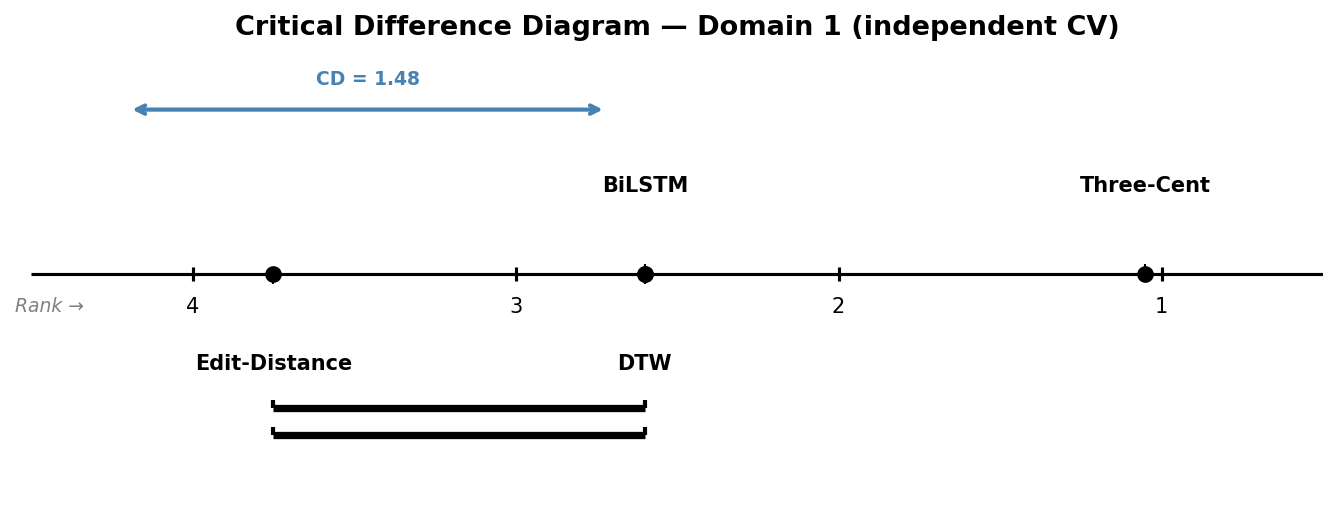
\includegraphics[width=\linewidth]{figures/cd_diagram_domain1_independent.png}
  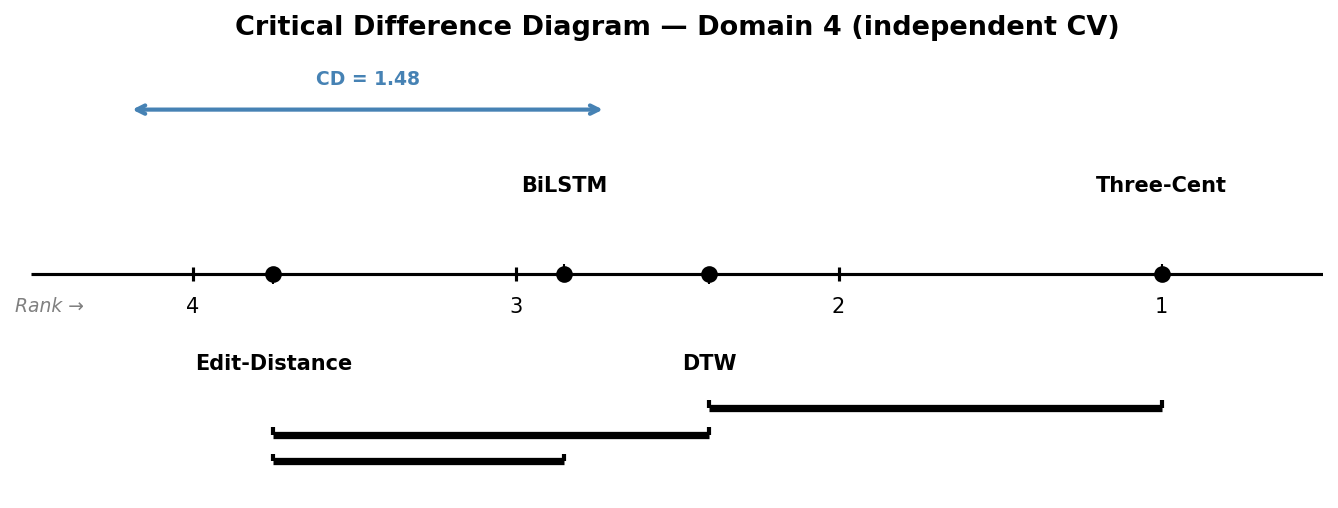
\includegraphics[width=\linewidth]{figures/cd_diagram_domain4_independent.png}
  \caption{Critical difference diagrams (Nemenyi, $\alpha = 0.05$) for
  domain~1 (top) and domain~4 (bottom) under user-independent CV\@.
  Methods are ranked from best (right, rank~1) to worst (left, rank~4).
  Horizontal bars connect methods whose rank difference does not exceed
  $\mathrm{CD} = 1.48$, i.e.\ whose performance is \emph{not} statistically
  distinguishable.}
  \label{fig:cd_diagrams}
\end{figure}
 
The diagrams lead to the following conclusions regarding~(Q3).
 
On \textbf{domain~1}, Three-Cents (avg.\ rank~1.05) stands isolated on the
right, connected to no other method: it is significantly better than DTW
(Wilcoxon adj-$p = 0.016$), Edit-distance (adj-$p = 0.012$) and BiLSTM
(adj-$p = 0.010$). DTW and BiLSTM share the same average rank (2.60) and are
not distinguishable from each other (adj-$p = 0.625$). The Wilcoxon--Holm
procedure does however separate Edit-distance from both DTW (adj-$p = 0.031$)
and BiLSTM (adj-$p = 0.023$), a difference the less powerful Nemenyi test
cannot detect.
 
On \textbf{domain~4}, Three-Cents (avg.\ rank~1.00) is again the sole
top-ranked method, significantly outperforming Edit-distance
(adj-$p = 0.010$), DTW (adj-$p = 0.012$) and BiLSTM (adj-$p = 0.008$). The
three remaining methods form a partially indistinct group: Edit-distance and
BiLSTM are not separable under either test, and DTW versus BiLSTM is also
non-significant (adj-$p = 0.238$). DTW does however significantly outperform
Edit-distance under Wilcoxon--Holm (adj-$p = 0.012$).
 
In summary, \textbf{Three-Cents is the only method that is statistically
superior to all others in both domains} under the user-independent protocol,
providing a clear and unambiguous answer to~(Q3). No other pairwise ordering
is consistently significant across both domains.
% ================================================================

% [To be completed.]

% ================================================================
\section{Conclusion}
\label{sec:conclusion}
% !TEX root = main.tex

This work implemented and compared four classifiers for 3D mid-air gesture
recognition on two domains from the dataset of Huang et al.~\cite{Huang2019}:
Dynamic Time Warping (DTW), Edit-distance on quantized symbolic sequences,
the Three-Cents ($3\mathbb{c}$) recognizer, and a Bidirectional LSTM.
The three research questions raised in the introduction can now be answered.

\paragraph{Q1 --- Classical vs.\ modern methods.}
Contrary to the common expectation that neural or more elaborate methods
should dominate, the Three-Cents recognizer --- a lightweight
resample--scale--translate template matcher --- achieves the highest
user-independent accuracy on both domains ($96.3\%$ on domain~1,
$95.1\%$ on domain~4), outperforming the BiLSTM by a margin of $11$--$25$
percentage points. This result highlights that the \emph{inductive bias} of
the method matters more than its computational complexity: Three-Cents
implicitly encodes the relevant invariances (translation, scale, partial
rotation) that mid-air gesture trajectories satisfy, whereas the BiLSTM must
learn these from a dataset too small to generalize reliably across users.
The dynamic-programming baselines (DTW, Edit-distance) occupy an intermediate
range, with DTW consistently outperforming Edit-distance in the
user-independent regime.

\paragraph{Q2 --- User-independent vs.\ user-dependent accuracy.}
The user-dependent setting yields systematically higher accuracy for every
method and every domain, as expected. The gap is most pronounced for
template-based methods: DTW and Edit-distance improve by up to $38$ percentage
points in the user-dependent regime, where training and test gestures share
the same motor style. Three-Cents and, to a lesser extent, the BiLSTM are
more robust to user shift: their user-dependent gains are smaller precisely
because their user-independent performance is already high. In user-dependent
mode, DTW, Edit-distance, and Three-Cents all approach saturation
($\geq 98\%$), confirming that the task becomes near-trivial once
within-user templates are available.

\paragraph{Q3 --- Is one method statistically superior?}
Yes. The Friedman test rejects the null hypothesis of equal expected ranks in
both domains ($p < 0.001$), and Nemenyi and Wilcoxon--Holm post-hoc tests
consistently identify Three-Cents as the sole method significantly better than
all others in the user-independent setting. No other pairwise ordering is
consistent across both domains.

\paragraph{Limitations and perspectives.}
The BiLSTM's underperformance is most plausibly a data-size effect: with
$\sim$1\,000 samples per domain, the network cannot learn the cross-user
invariances that Three-Cents enforces by design. Training on a larger,
more diverse cohort --- or augmenting the dataset with synthetic inter-user
style transfers --- would likely narrow this gap considerably. The ablation
study further revealed that PCA applied without prior normalization can
degrade performance for Edit-distance, a methodological pitfall worth
flagging for practitioners. Finally, the confusion analysis showed that
all remaining errors are geometrically motivated: the Pyramid--Cylindrical
Pipe and digit~0--8 boundaries are the hardest pairs and could be targeted
with class-specific augmentation or cost-sensitive training.

More broadly, this project illustrates that well-designed, geometry-aware
feature engineering can rival or surpass end-to-end learned representations
when labeled data is scarce --- a conclusion that remains practically relevant
beyond the specific gesture recognition setting studied here.





% ----------------------------------------------------------------
\bibliographystyle{plain}
\bibliography{references}

\section*{IA Disclosure}
% !TEX root = main.tex
\addcontentsline{toc}{section}{Use of Generative AI Tools}
This report was produced with the assistance of a generative AI
language model (Anthropic Claude) used as a productivity and
analytical support tool. Specifically, AI assistance was used for
the following tasks:
\begin{itemize}
  \item \textbf{Code generation and debugging.}
  The Python pipeline implementing the four classifiers
  (DTW, Edit-distance with $k$-means vector quantization,
  Three-Cents, and BiLSTM), the nested cross-validation
  infrastructure, the hyperparameter grid search, the
  preprocessing utilities (z-score normalization, PCA),
  and the statistical assessment routines (Friedman,
  Nemenyi, Wilcoxon--Holm) were developed with AI-assisted
  code generation, iterative debugging, and structural review.
  \item \textbf{Methodological cross-checks.}
  The design of the nested inner/outer cross-validation
  protocol, the choice of statistical tests for comparing
  multiple classifiers across folds, and the data-leakage
  prevention strategy (fitting all preprocessing exclusively
  on the inner training set) were refined through AI-assisted
  discussion against the relevant literature.
  \item \textbf{Ablation study design.}
  The systematic ablation grid isolating the effects of
  normalization and PCA across the 80 (method, domain,
  CV mode, preprocessing) configurations was structured
  with AI assistance. The interpretation of the resulting
  interactions --- in particular the normalization $\times$ PCA
  effect for edit-distance and the intrinsic robustness of
  Three-Cents --- was made by the authors.
  \item \textbf{LaTeX drafting and structure.}
  Section drafts, table formatting, mathematical notation,
  figure design (LSTM cell, BiLSTM architecture, critical
  difference diagrams), and the overall report structure
  were refined with AI assistance. All analytical content,
  interpretations, and conclusions were reviewed, validated,
  and approved by the authors.
  \item \textbf{Critical review.}
  The AI tool was used to perform a simulated critical
  evaluation of the report prior to submission, identifying
  inconsistencies between the text and the experimental
  grids, gaps in the discussion of the research questions
  (Q1--Q3), and missing references to foundational works.
\end{itemize}
All quantitative results reported in this document
(accuracies, standard deviations, p-values, confusion
matrices, hyperparameter selections) were produced by
running the Python pipeline on the gesture datasets of
Huang et al.~\cite{Huang2019} and verified by the authors
against the generated raw CSV output files. The AI tool
did not execute the pipeline directly and did not produce
any numerical results autonomously. Responsibility for
the analytical choices, model implementations, statistical
methodology, and conclusions rests entirely with the authors.
\label{sec:ia_disclosure}


\input{page_de_fin.tex}

\end{document}